\documentclass[oneside]{scrbook}
\setkomafont{author}{\scshape}
\usepackage{blindtext}
\usepackage[utf8]{inputenc}
\usepackage{listings}
\usepackage{graphicx}
\usepackage{mathtools}
\DeclarePairedDelimiter{\ceil}{\lceil}{\rceil}
\usepackage{amssymb}

\title{Avancerede Datastrukturer}
\subtitle{Projekt 1 DM803}
\author{Gabriella Juhl Jensen\thanks{CPR nr.: 160396, e-mail: gajen16} \and Samuel Valdemar Grange\thanks{CPR nr.: 081097, e-mail: sagra16} }
\subject{Skip lists and Scapegoat Trees}

\begin{document}

\maketitle
\section*{Introduction}
For this project our goal was to implement the SplitList and ScapeGoat structures and analyse their performance.
We have chosen to implement the structures in Scala.
Since Scala is a more functional language than what one traditionally would choose for low level, mutable algorithms such as these,
the underlying implementations are structured differently.
This is a consequence of choosing pattern matching, null-safe, type-safe and immutable constructs as the building blocks rather than traditional imperative methods.
\\

Counting comparisons is a bit more complicated than with a traditional language, since some pattern matching or std-lib functions might "count" as a comparison.
Because of this we have chosen to be a bit pessimistic about counting;
we count a comparison when in doubt.

It should also be noted that some of the functions might have a constant which is not exactly the same as the describe algorithm, but the complexity is the same.

Finally we have used tail-recursion and recusive algorithms much more vigorously than the described algorithms to avoid side-effectful things such as while loops.

\chapter{Split list}
Complexity wise the interesting aspect of skip list is the trade off made by adjusting the $p$ value.
The $p$ value is a probability threshold that decides whether a node should grow larger or not.

This $p$ value, is actually a knob that trades traversal speed with update speed.
Updating a node which has height $1$ is simple, because it only has one parent and one child.
Traversing a linked list has complexity $\mathcal{O}(n)$, which skip list significantly improves by introducing these "highways".

We expect that the worst-case can be invoked for insertion and deletion by always picking a node that near the end of the list.
"near" means as far back as possible while having a height that equals the levelcap.

We expect that by decreasing the $p$ value we will see increases in deletion and insertion comparisons, and reductions in search comparisons.

Tuning wise it would seem most appropriate to have a small $p$ if fast searches are required, and having a medium sized $p$ for many insertions/deletions.\
A small $p$ for many "highway" levels to do fast lookups.\
A medium sized $p$ so the "highways" have a size that allows semi-optimal lookup, and not too small so the sizes of the

\section*{Additional notes}
It should be noted that when running the splitlist from the CLI we use an algorithm to determine the levelcap:
$$\ceil{log_{1/p}(n)}$$
Where n is the maximum amount of elements ever present in the structure.\\
Having $129$ elements and a $p$ of $0.5$:\\
$0.5$ is a reduction factor $r$ of $2$ or $\frac{1}{p}$.\\
We must find a height such that all elements will "fit".
We must find $x$ that satisfies $x \in \mathbb{N}$ which also satisfies $n = \Big( \frac{1}{p} \Big)^{z}$ and $n \leq \Big( \frac{1}{p} \Big)^{x}$
for some $x = \ceil{z}$.
$$129 = 2^{\ceil{z}}$$
$$log_2(129) = \ceil{z}$$
$$7.011... = \ceil{z}$$
$$x = 8$$


\section{Investigateted}
\subsection{Avarage shearch complexity}
\subsection{Variation in shearch complexity}
\section{Test}
\chapter{Scapegoat Trees}
Scapegoat like the splitlist has a "tuning-knob" $\alpha$, which allows us tune the structure to the expected data.
This $\alpha$ controls how "unbalanced" the tree is allowed to be, until a rebuild is forced.

The minimum value of this $\alpha$ is $0.5$, which will mean that the tree will stay entirely balanced.
Conversely an $\alpha$ which is close to $1$ will allow a more unbalanced tree.
\\\\
Obviously $\alpha = 0.5$ will result in very fast lookups, as the visits will always be the tree height, or $\mathcal{O}(log(n))$.
This will come with the consequence that changes to the tree might very well invoke a rebuild, which is expensive.
\\\\
The other extreme $\alpha = 0.99...$ will ensure that the insertion time and deletion is relatively fast, but the lookup time will be $\mathcal{O}(n)$;
all nodes only having one child, potentially created by the insertion sequence $1,2,3... n$.
\\\\
An overall good $\alpha$ must be somewhere in between.

\section*{Testing}
The unit tests are contained freely in the main class, and can be invoked by supplying the appropriate command-line arguments.\\
We have tested the example input given in the project description:\\
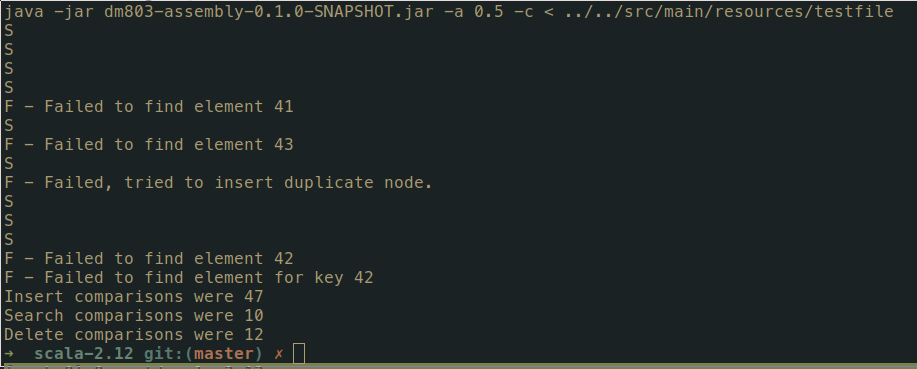
\includegraphics[scale=0.5]{kimtest.png}

\section*{Notes for runtime}
The code given will compile with a working scala compiler of version $> 2.10$.\\
A pre-compiled jar and bytecode graal compiled version has been given.\\
The requirements for running the jar is simply a Java-jre installation (tested with java 11 and openjdk:8).\\
A Dockerfile has also been supplied (in some disaster case):
\begin{lstlisting}
docker build -t test .
docker run -i test -p 0.5 < some_file
\end{lstlisting}


\end{document}
